\documentclass{article}
\usepackage[T1]{fontenc}
\usepackage{lmodern}
\usepackage{graphicx}
\usepackage{url}

\begin{document}

	\part*{Gebruiker-gids}
	
	\section{Introductie}
	Domotica is een programma die het beheers van energie in een gebouw controleert. Elke kamer heeft een steward die verschillende devices beheert, en de central-unit controleert de verschillende stewards. Deze stewards kunnen berichten zenden naar hun devices. Een device bestaat uit sensoren en actuatoren die diverse elementen (temperatuur, licht-intensiteit...) kunnen meten en aanpassen.
	
	\begin{description}
		\item[\ref{main-menu} Hoofdscherm] : het overzicht-scherm van de applicatie.
		\item[\ref{add-device} Device Toevoegen] : het scherm waarmee een nieuw type device toegevoegd kan worden.
		\item[\ref{add-steward} Steward Toevoegen] : het scherm waarmee een nieuwe steward toegevoegd kan worden.
	\end{description}
	
	\section{Hoofdscherm}
	\label{main-menu}
	Dit is het overzicht scherm van het domotica-programma. Hier kan de toestand van de verschillende stewards bekeken worden en de geschiedenis van hun metingen.
	
	\newpage
	
	\begin{figure}
		\begin{center}
			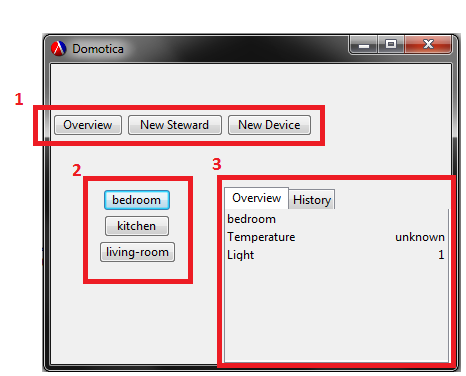
\includegraphics{screenshot/main-menu.png}
		\end{center}
		\caption{Het main menu.}
	\end{figure}
	
	\begin{enumerate}
		\item Hier is het mogelijk om naar de verschillende menus te navigeren.
		\item Een lijst van de bestaande stewards.
		\item Een overzicht van de geselecteerde steward.
	\end{enumerate}
	
	\section{Device Toevoegen}
	\label{add-device}
	In dit menu is het mogelijk om een nieuw type device toevoegen. Een device bestaat uit een aantal sensoren en actuatoren die gekozen kunnen worden uit de lijst of toegestaande sensoren en activatoren. Een steward kan alleen bestaande types devices beheersen, deze moeten dus op voorrand in dit menu toegevoegd worden.
	
	\newpage
	\begin{figure}
		\begin{center}
			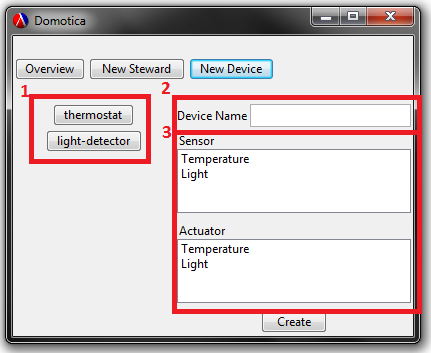
\includegraphics{screenshot/new-device.png}
		\end{center}
		\caption{Voeg een nieuw device toe.}
	\end{figure}
	
	\begin{enumerate}
		\item Een lijst van de bestaande type devices.
		\item Vul hier de naam van het nieuwe device in.
		\item Kies tussen de toegelaten sensoren en activatoren.
	\end{enumerate}
	
	\section{Steward Toevoegen}
	\label{add-steward}
	In dit menu is het mogelijk om nieuwe stewards toe te voegen aan het domotica-programma (\ref{new-steward}). Een steward beheert een aantal devices, de serial-nummers van deze devices worden gevraagd zodat de steward ermee kan communiceren (\ref{new-steward-confirmation}).
	
	\begin{figure}
		\begin{center}
			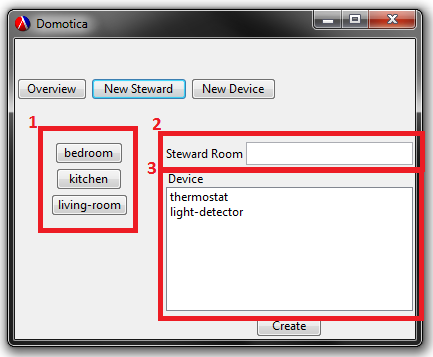
\includegraphics{screenshot/new-steward.png}
		\end{center}
		\caption{Voeg een nieuwe steward toe.}
		\label{new-steward}
	\end{figure}
	
	\begin{enumerate}
		\item Een lijst van de bestaande stewards.
		\item De kamer waarin de nieuwe steward zal opereert (maar een steward per kamer).
		\item Voeg devices toe die in deze lijst inbegrepen zijn.
	\end{enumerate}
	
	\begin{figure}
		\begin{center}
			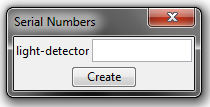
\includegraphics{screenshot/new-steward-confirmation.png}
		\end{center}
		\caption{Vul de serial-numbers van de gekozen devices}
		\label{new-steward-confirmation}
	\end{figure}

\end{document}